
\Section{Lightning network}
One of the biggest problems facing bitcoin is scalability. At time of writing
onchain transactions is capped at about $\approx 7$ T/s (transactions er second).\cite{scaling}
This has to do with network propagation and the hard cap on block sizes, a block
can only contain so many transactions before it is full. There are a couple of
propsed solutions to this however, and lightning is one of them.

Lightning network is a relatively recent development in the bitcoin community.
Many types of experimental transactions have been known for a long time. But in
January of 2016 a white paper was released detailing a brand new type.\cite{lightningnetwork_2019}
It showed that with a few changes to the bitcoin protocol a new type of
transaction that opens a channel between two parties ca be made. In this channel
an unlimited number of transactions could be potentially made between the two
parties. \cite{lightningnetwork_2019}

\begin{figure}[H]
	\centering
	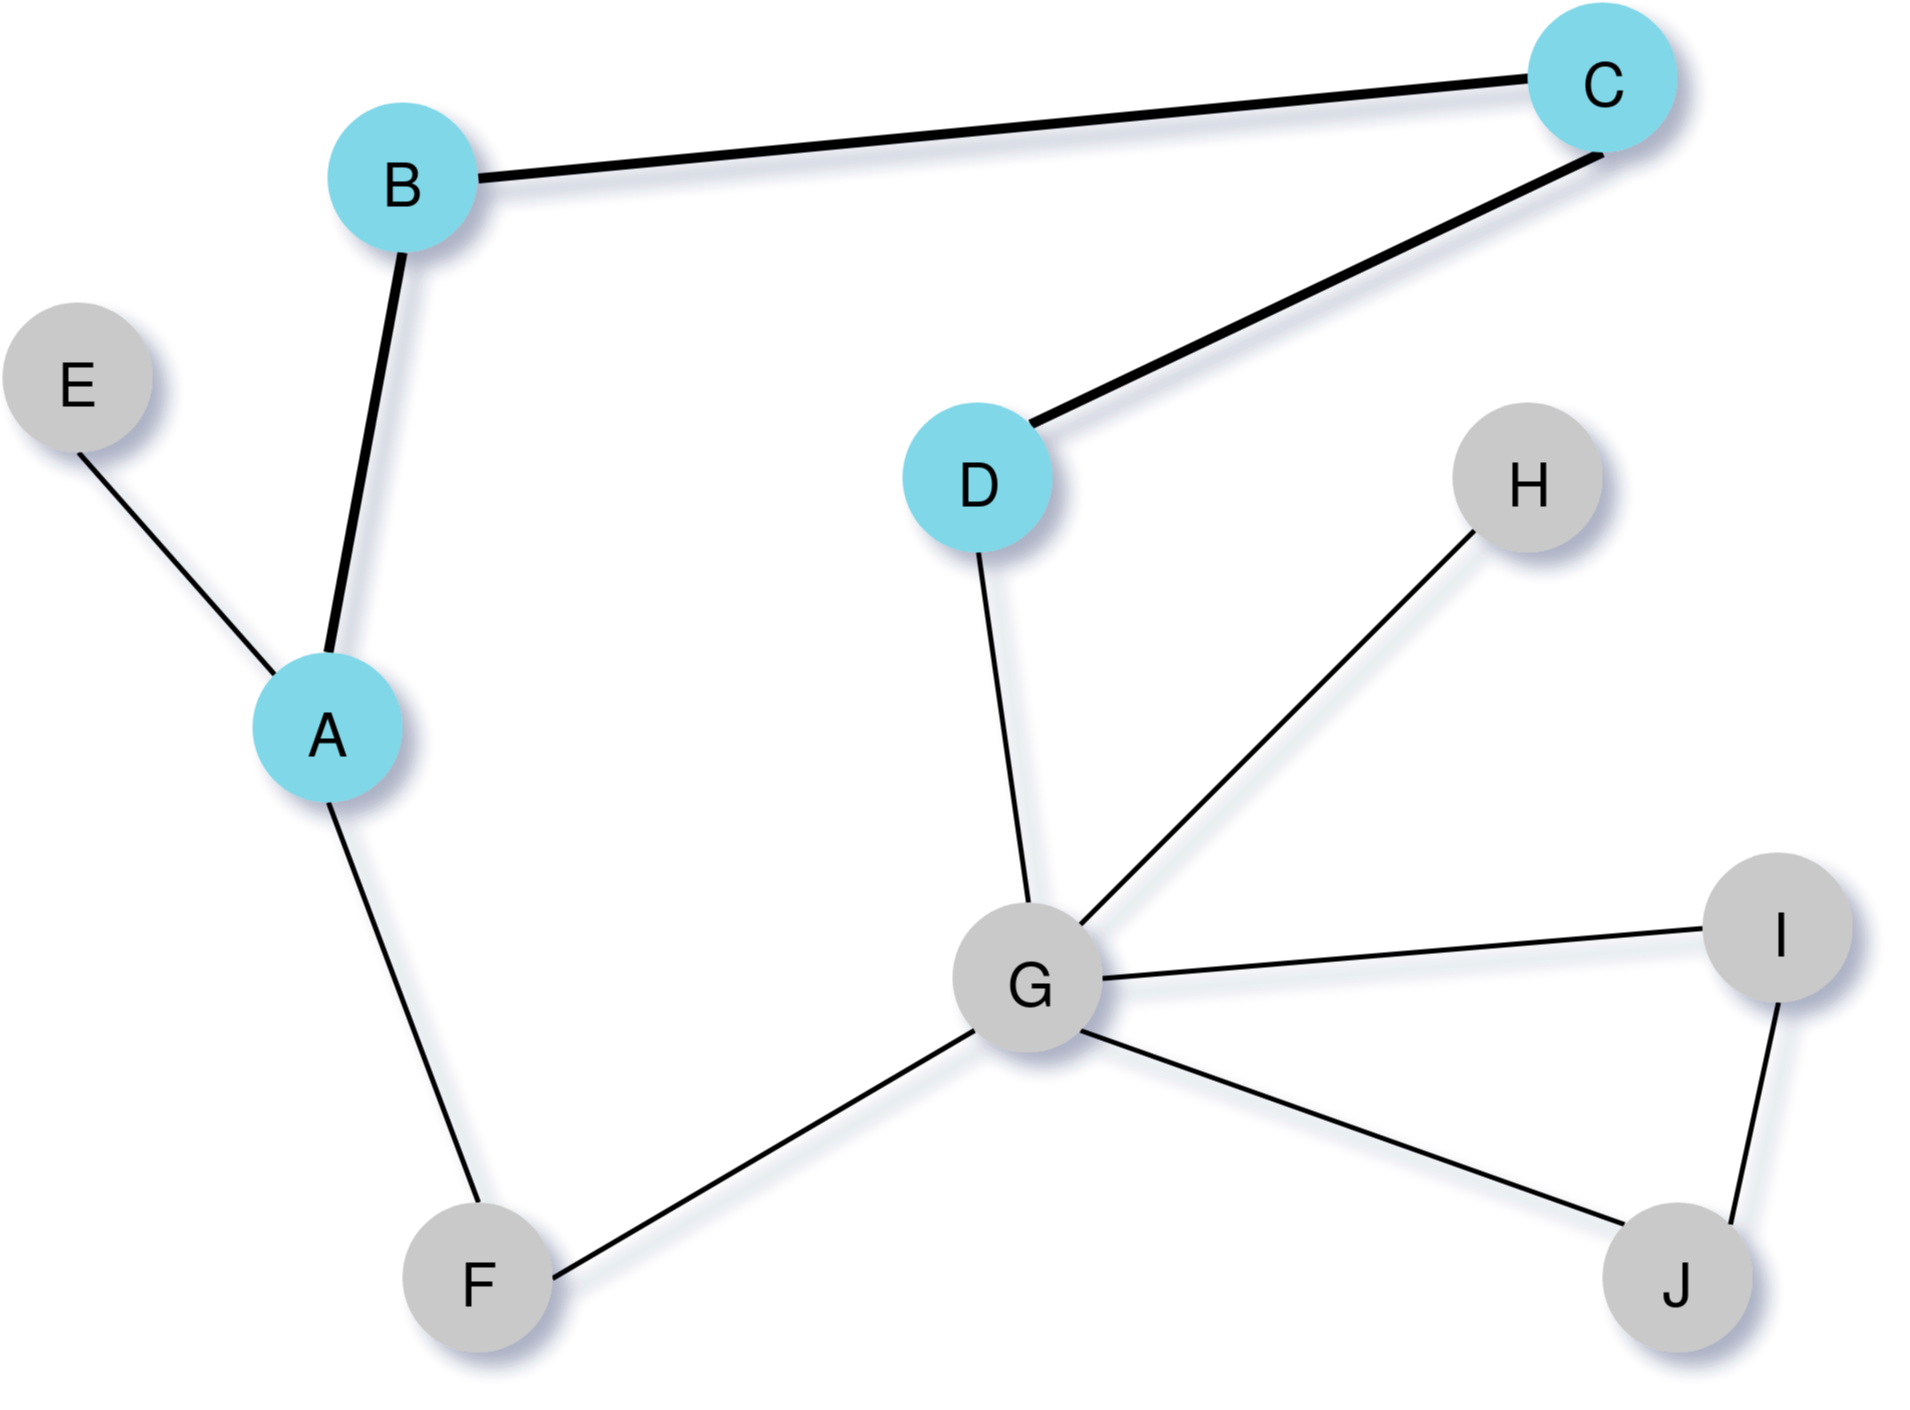
\includegraphics[width=0.70\textwidth]{introduction/images/mesh_network.png}
	\caption{A basic overview of a lightning network, each node represent someone
	and each edge represents a channel between two people.}
	\label{fig:blockchain3}
\end{figure}

The name lightning network most likely a combination of lightning, as in
lightning fast transactions. And network from the network that is formed by
participants and their channels. One very useful feature of lightning network
is that two parties do not need to have direct channel between them to be able
to transact. Transactions can safely and atomically travel through the network
via other participants, as long as there is a path between the two and there is
enough funds in all the channels in between.\cite{lightningnetwork_2019}
